%% Copyright 2019 Bernd Haberstumpf
%% License: CC BY-NC
% !TeX spellcheck = de_DE
\newsection{Charakter Erschaffung}

Die F"ahigkeiten und Eigenschaften eines Charakters werden bei der Erstellung des Charakters festgelegt und auf seinem Charakterdatenblatt festgehalten. Das Charakterdatenblatt ist am Ende dieses Kapitel angeh"angt. Es kann auch separat im Internet heruntergeladen werden. Ein entsprechender Link findet sich unter Quellenangaben am Ende des Buchs. Charakterdatenbl"atter sind "ublicherweise, wie auch bei diesem Regelsystem, in englischer Sprache verfasst.

\newsubsection{Allgemeine Daten}
\begin{column}[l]{0.48}
    Das Charakterdatenblatt beginnt mit allgemeinen Daten wie Name, Geschlecht (\stat{GENDER}), Rasse (\stat{RACE}), Alter (\stat{AGE}), Talente und Schw"achen (\stat{MERITS \& FLAWS}). Die verf"ugbaren Rassen sind im n"achsten Kapitel beschrieben.
\end{column}
\begin{column}[r]{0.52}
    \centering
    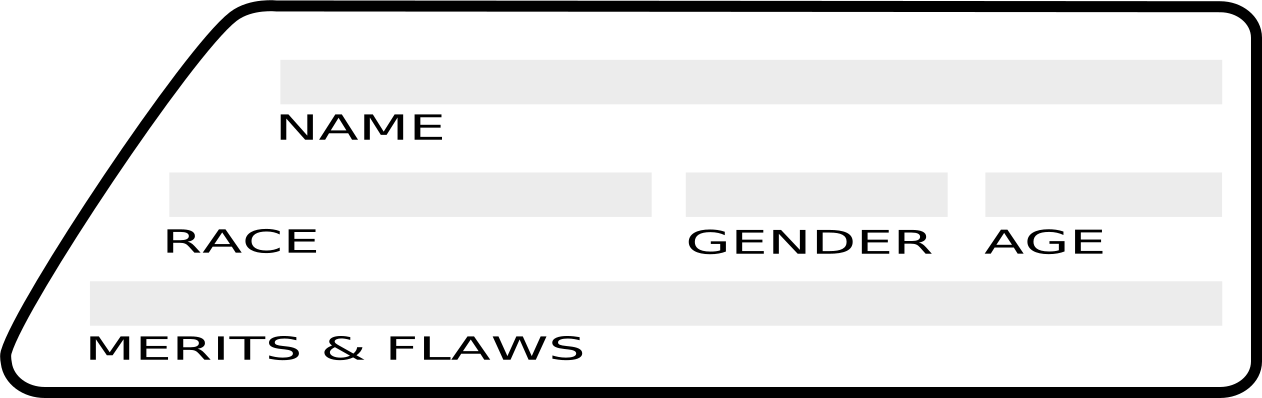
\includegraphics[width=0.95\textwidth]{images/character_base_stats.png}
    \medskip   
\end{column}
\medskip

\sheet{Name, Geschlecht, Rasse und Alter k"onnen durch den Spieler frei gew"ahlt werden.}

Die Charaktere sind "ublicherweise zwischen 30 und 50 Jahre alt. Ein deutlich niedriges oder deutlich h"oheres Alter kann negative Einfl"usse auf k"orperliche Verfassung oder die F"ahigkeiten des Charakters haben. Eine Einschr"ankung kann unter \stat{MERITS \& FLAWS} auf dem Charakterdatenblatt notiert werden.

\sheet{Um die Charaktere dar"uber hinaus lebhafter zu gestalten, kann eine Schw"ache, ein Flaw, f"ur den Charakter festgelegt werden.}

\newsubsection{Hintergrund}
\begin{column}[l]{0.52}
    Die \cref{sec:character} eingef"uhrten Hintergr"unde des Charakters werden im Feld \stat{BACKGROUND} notiert. Die Hintergr"unde beschreiben den individuellen Lebensweg eines Charakters.
\end{column}
\begin{column}[r]{0.48}
    \centering
    
\includegraphics[width=0.80\textwidth]{images/character_background.png}    
\end{column}

\medskip
Hintergr"unde sind jeweils einem der \emph{Attribute} \stat{[B]ODY}, \stat{[E]MPATHY} und \stat{E[D]UCATION} zugeordnet. Die einem Attribut zugeordneten St"arken, die sogenannten \emph{F"ahigkeiten}, beziehen sich immer auf entsprechende Hintergr"unde.

\sheet{Das Attribut, auf das sich ein Hintergrund bezieht, wird in der Hintergrundbeschreibung unter \stat{BACKGROUND} mit \stat{[B]}, \stat{[E]} oder \stat{[D]} erg"anzt.}

\medskip
\begin{ruleexample}
    Bei einem Agenten der Cynarian Corporation findet sich z.B. der \stat{BACKGROUND} "`Cynarian Agent [E]"', wobei \stat{[E]} das Attribut \stat{[E]MPATHY} kennzeichnet. St"arken im Bereich des Attributs sind auf das Umfeld eines Cynarian Agenten beschr"ankt.
\end{ruleexample}

\newsubsection{Attribute und F"ahigkeiten}
Die St"arken eines Charakters werden aufgeteilt nach den Attributen \stat{[B]ODY}, \stat{[E]MPATHY} und \stat{E[D]UCATION} gruppiert. Die Attribute repr"asentieren die Grundf"ahigkeiten des Charakters. Unter den Attributen sind die St"arken, die sogenannten \emph{F"ahigkeiten} des Charakters gruppiert. Jedem Attribut sind jeweils drei F"ahigkeiten zugeordnet. 

Neben einer F"ahigkeit sind jeweils die Anzahl der W"urfel notiert, die f"ur eine Aktion, die mit der F"ahigkeit ausgef"uhrt werden kann, zur Verf"ugung stehen. F"ur die F"ahigkeiten eines Charakters stehen bis zu drei W"urfel zur Verf"ugung, die durch die Boxen neben den F"ahigkeiten  festgehalten werden. 

Die erste bereits ausgef"ullte Box neben jedem Attribut und jeder F"ahigkeit symbolisiert, dass f"ur beliebige Aktionen mindestens ein W"urfel zur Verf"ugung steht.

Ein gef"ulltes Dreieck rechts neben einem Attribut zeigt an, dass f"ur die darunterliegenden F"ahigkeiten bis zu drei W"urfel zur Verf"ugung stehen k"onnen. Bei Attributen mit leerem Dreieck stehen maximal zwei W"urfel f"ur eine F"ahigkeit zur Verf"ugung.

\sheet{Bei Mutanten ist das Dreieck bei \stat{BODY} ausgef"ullt. Norms k"onnen frei zwischen \stat{EMPATHY} und \stat{EDUCATION} w"ahlen.} 

\sheet{Bei der Charaktererstellung k"onnen f"ur F"ahigkeiten insgesamt 6 Punkte vergeben werden. F"ur jeden ausgegebenen Punkt kann eine Box neben einer F"ahigkeit ausgef"ullt und damit ein zus"atzlicher W"urfel erworben werden.}

\newsubsection{F"ahigkeiten}
Die 9 F"ahigkeiten beschreiben grob die St"arken eines Charakters. Inwieweit eine F"ahigkeit auf eine Aktion anwendbar ist, liegt im Ermessen des Spielleiters. Die F"ahigkeiten sind bewusst allgemein gehalten und k"onnen sich "uberschneiden. Der Spieler beschreibt zun"achst die Aktion, die er ausf"uhren will. Anschlie\3end bestimmen der Spieler und der Spielleiter gemeinsam, welche F"ahigkeit am besten anwendbar ist.

Die F"ahigkeiten eines Charakters beziehen sich immer auf einen entsprechenden Hintergrund. Die Eigenschaft \stat{Dexterity} eines Piloten erm"oglicht es ihm, bei Flugman"overn zus"atzliche W"urfel zu werfen, w"ahrend ein Schiffstechniker mit \stat{Dexterity} seine St"arken bei der Reparatur und Modifikation eines Raumschiffs ausspielen kann.

Die folgenden Beschreibungen geben Beispiele f"ur Anwendungsgebiete der F"ahigkeiten. Sie sind jedoch nicht dazu gedacht, alle Anwendungsm"oglichkeiten abzudecken.

\medskip
\begin{column}[l]{0.55}
    F"ur das Attribut \stat{BODY}, das die k"orperlichen Eigenschaften des Charakters darstellt, stehen folgende F"ahigkeiten zur Verf"ugung:
\end{column}
\begin{column}[r]{0.45}
    \centering
    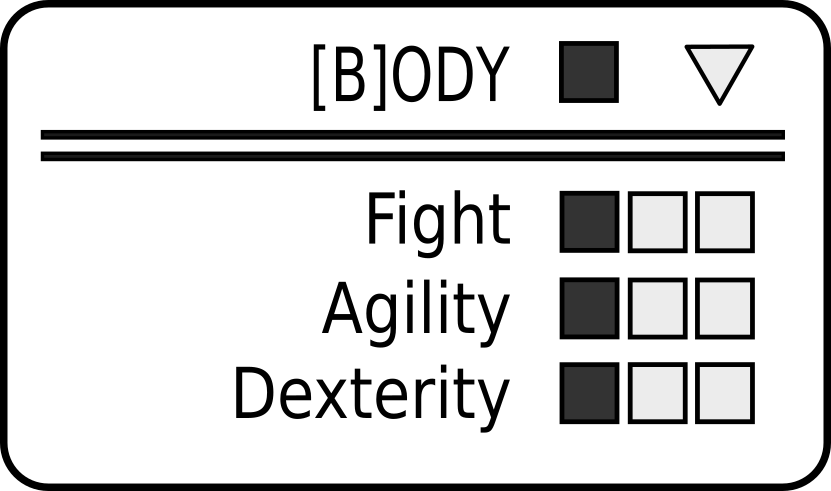
\includegraphics[width=0.80\textwidth]{images/character_body.png}
\end{column}

\begin{description}
    \item[\stat{Fight}] stat{Fight} findet im Nah- und Fernkampf Anwendung. Es umfasst nicht nur den Angriff, sondern auch die 
        Verteidigung, jedoch z.B.~nicht das Hakenschlagen bei einer Flucht. Der Hintergrund bestimmt, in welcher Kampfart und mit welchen Waffen ein Charakter ausgebildet bzw.~ge"ubt ist.
    \item[\stat{Agility}] \stat{Agilit"at} umfasst Sportlichkeit, Fingerfertigkeit und die Nutzung aller Sinnesorgane. 
    
        Es kann im Kampf f"ur eine Flucht, das Wegtauchen in eine Deckung, aber auch zum Ausweichen von Schl"agen genutzt werden. F"ur das Ausweichen von Schl"agen k"onnte jedoch auch wiederum \stat{Fight} genutzt werden.

        Die Fingerfertigkeit bei Reparaturen "uberschneidet sich mit den handwerklichen F"ahigkeiten, f"ur die auch \stat{Dexterity} genutzt werden kann.
    
        \stat{Agility} umfasst die Sinneswahrnehmungen Sehen, Tasten, Riechen und F"uhlen. Es kann z.B.~beim Durchsuchen von R"aumen angewendet werden. 
    \item[\stat{Dexterity}] \stat{Dexterity} umfasst handwerkliche F"ahigkeiten, die Bedienung von schwerem Ger"at sowie die Steuerung von 
        Fahrzeugen und Schiffen. Der spezifische Hintergrund des Charakters bestimmt die Auspr"agung und Anwendungsbereiche dieser F"ahigkeit.
\end{description}

\medskip
\begin{column}[l]{0.55}
    Das Attribut \stat{EMPATHY}, gruppiert alle sozialen F"ahigkeiten des Charakters. Es stehen folgende F"ahigkeiten zur Verf"ugung:
\end{column}
\begin{column}[r]{0.45}
    \centering
    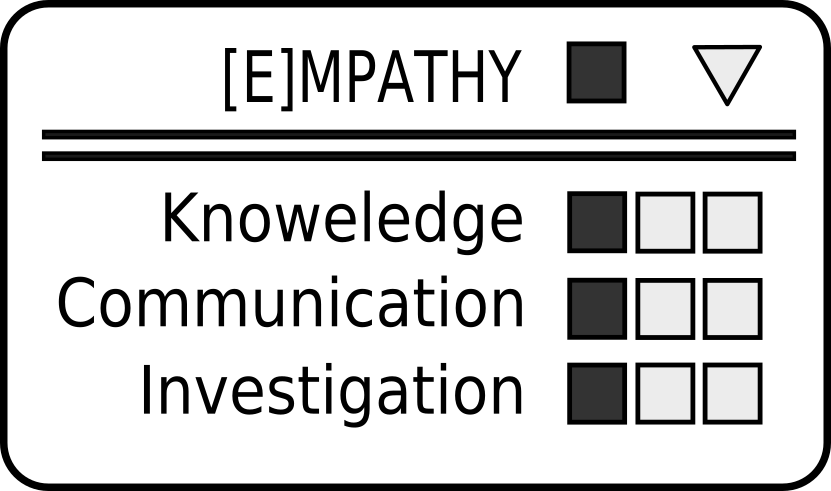
\includegraphics[width=0.80\textwidth]{images/character_empathy.png}
\end{column}

\begin{description}
    \item[\stat{Knowledge}] \stat{Knowledge} beschreibt das Allgemeinwissen des Charakters. Dieses Wissen ist in der Regel auf den 
        Kulturkreis beschr"ankt, in dem der Charakter aufgewachsen ist. Beispielsweise hat ein auf dem Mars aufgewachsener Charakter nur begrenztes Wissen "uber die russische Geschichte, es sei denn, er hat sich gezielt damit besch"aftigt.

        Ein Charakter mit einem hohen \stat{Knowledge}-Wert ist stets gut informiert und kennt die neuesten Entwicklungen, die f"ur sein Umfeld relevant sind.
    \item[\stat{Communication}] \stat{Communication} beschreibt die Kommunikationsf"ahigkeit des Charakters, also wie gut er mit anderen 
        Personen interagieren kann.

        Diese F"ahigkeit umfasst auch, wie gut der Charakter andere einsch"atzen, sich in sie hineinversetzen und sie gegebenenfalls manipulieren kann.

        \stat{Communication} umfasst die Kontaktnetzwerke des Charakters. Ein hoher \stat{Communication}-Wert erh"oht die Wahrscheinlichkeit, dass der Charakter jemanden kennt, der ihm bei einer Aufgabe helfen kann.
    \item[\stat{Investigation}] \stat{Investigation} bestimmt, wie effektiv ein Charakter Nachforschungen anstellen kann. Diese F"ahigkeit 
        erm"oglicht es ihm, Verborgenes zu entdecken.

        \stat{Investigation} findet sowohl in der realen als auch in der virtuellen Welt Anwendung.
\end{description}

\medskip
\begin{column}[l]{0.55}
    F"ur das Attribut \stat{EDUCATION}, das die Bildung und Fachkenntnisse des Charakters repr"asentiert, stehen folgende F"ahigkeiten zur Verf"ugung:

\end{column}
\begin{column}[r]{0.45}
    \centering
    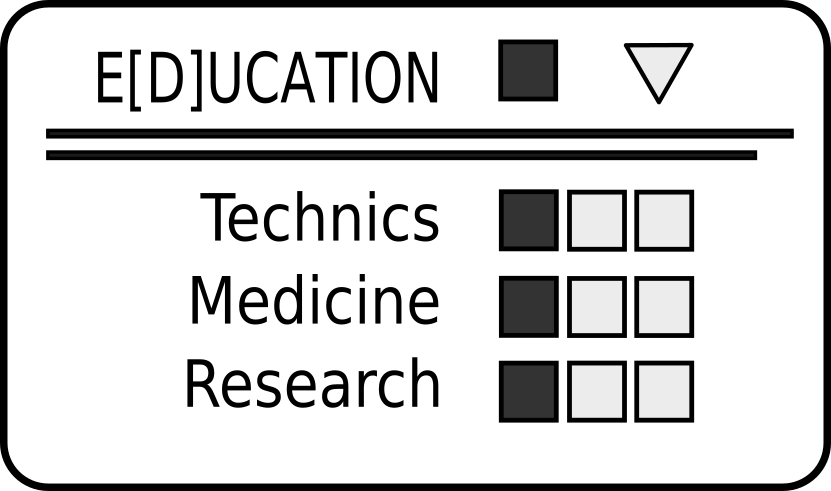
\includegraphics[width=0.80\textwidth]{images/character_education.png}
\end{column}

\begin{description}
    \item[\stat{Technics}] \stat{Technics} beschreibt das Wissen und Verst"andnis f"ur technische Systeme. Je nach \stat{BACKGROUND} kann das beispielsweise Raumfahrttechnik, Computertechnik oder "Ahnliches umfassen.
    \item[\stat{Medicine}] \stat{Medicine} beinhaltet medizinisches Wissen, einschlie\3lich Pharmakologie und Drogenkunde. 
    
        Diese F"ahigkeit umfasst T"atigkeiten als Arzt oder Sanit"ater sowie das Verst"andnis f"ur Abl"aufe in medizinischen Einrichtungen wie Krankenh"ausern. 
        
        Die Anwendung dieser F"ahigkeit ist abh"angig vom medizinischen \stat{BACKGROUND} des Charakters.
    \item[\stat{Research}] \stat{Research} umfasst Forschungskompetenz in den Fachgebieten, mit denen der Charakter vertraut ist, basierend 
        auf seinem \stat{BACKGROUND}.
\end{description}

\underline{Anmerkung:} Wie die Beschreibungen zeigen, ist die Anwendbarkeit der F"ahigkeiten des Attributs \stat{EDUCATION} besonders abh"angig vom \stat{BACKGROUND} des Charakters. Die F"ahigkeit \stat{Research} kann beispielsweise nicht in allen wissenschaftlichen Bereichen angewendet werden, sondern nur in jenen, f"ur die der Charakter ausgebildet wurde.

\medskip
\begin{ruleexample}
    Die Gruppe fl"uchtet von einer Orbitalstation mit einem Wartungsshuttle, um sich auf einem Mond zu verstecken. Das Haupttriebwerk des Shuttles ist au\3er Betrieb. Um das Shuttle zu beschleunigen und auf die richtige Flugbahn zu bringen, wird ein Parabelflug geplant, der die Gravitation mehrerer Meteore in der Umgebung ausnutzt. Hierf"ur m"ussen alle Charaktere zusammenarbeiten:

\begin{description}
        \item[Celine ({Hintergrund Mathematikerin [D]})] Celine berechnet mithilfe ihrer mit drei W"urfeln ausgepr"agten F"ahigkeit 
            \stat{Research} eine Flugbahn.
        \item[Henk ({Hintergrund Navigator [E)})] Henk nutzt die von Celine berechnete Flugbahn, um mit seiner F"ahigkeit \stat{Knowledge} 
            die Flugparameter zu bestimmen.
        \item[Tom ({Hintergrund Shuttlepilot [B]})] Tom, der Pilot, bringt mit seiner F"ahigkeit \stat{Dexterity} das Shuttle mit den 
            Man"overd"usen aus dem Raumdock und folgt den von Henk bestimmten Flugparametern, um das Shuttle auf die richtige Flugbahn zu setzen.
    \end{description}
\end{ruleexample}

\newsubsection{Waffen}
\begin{column}[l]{0.55}
    Im Bereich \stat{WEAPONS} werden die Waffen eingetragen, die dem Charakter zur Verf"ugung stehen. Spielercharaktere verf"ugen "ublicherweise "uber eine halbautomatische Handfeuerwaffe. Abh"angig von der Profession des Charakters k"onnen zus"atzliche Waffen zur Verf"ugung stehen. Die Auswahl der Waffen ist mit dem Spielleiter abzustimmen.
\end{column}
\begin{column}[r]{0.45}
    \centering
    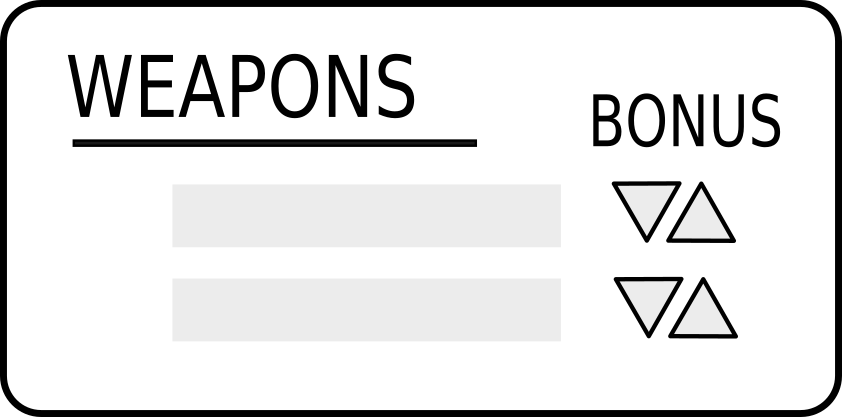
\includegraphics[width=0.80\textwidth]{images/character_weapons.png}
\end{column}
\medskip

Eine Auswahl an Waffen, beschrieben \cref{sec:weapons}, steht zur Verf"ugung. Dort sind auch die speziellen Eigenschaften der Waffen notiert. Wie Waffen im Rahmen des Regelwerks gruppiert werden findet sich \cref{sec:heavyweapons}.

Auf dem Charakterblatt sind neben jeder Waffe zwei Dreiecke angegeben. Bei Waffen, die schwer zu beherrschen sind, wird das nach unten zeigende Dreieck ausgef"ullt. Bei einer solchen Waffe werden Angriffe mit einem W"urfel weniger gew"urfelt (\emph{Malus}), jedoch mindestens mit einem W"urfel. Bei Waffen, die eine erh"ohte Trefferchance aufweisen, wird das nach oben zeigende Dreieck ausgef"ullt (\emph{Bonus}). Bei diesen Waffen wird mit einem zus"atzlichen W"urfel gew"urfelt.

\newsubsection{K"orperpanzerung}
\begin{column}[l]{0.55}
    Im Bereich \stat{ARMOR} werden die dem Charakter zur Verf"ugung stehenden K"orperpanzerungen und au\3ergew"ohnliche Kleidungsst"ucke wie individuelle Raumanz"uge eingetragen.
\end{column}
\begin{column}[r]{0.45}
    \centering
    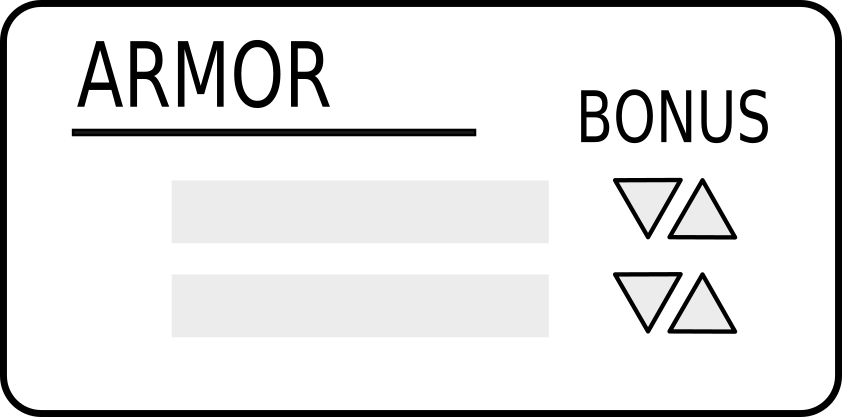
\includegraphics[width=0.80\textwidth]{images/character_armor.png}
\end{column}
\medskip

Eine Auswahl an K"orperpanzerungen ist \cref{sec:panzerung} gelistet. Dort sind auch die speziellen Eigenschaften der Panzerungen beschrieben.

Neben der Kleidung sind auf dem Charakterblatt zwei Dreiecke angegeben. Bei Kleidung, die den Charakter stark behindert und gleichzeitig unzureichenden Schutz bietet, wird das nach unten zeigende Dreieck ausgef"ullt. Bei solch einer Kleidung steht f"ur die Verteidigung ein W"urfel weniger zur Verf"ugung (\emph{Malus}). Bei Panzerungen, die den Charakter "uberdurchschnittlich gut sch"utzen, wie z.B. ein Servopanzer, wird das nach oben zeigende Dreieck ausgef"ullt. Bei einer solchen K"orperpanzerung steht ein W"urfel mehr zur Verf"ugung (\emph{Bonus}).

\newsubsection{Inventar}
\begin{column}[l]{0.55}
    Im Bereich \stat{INVENTORY} sind die pers"onlichen Habseligkeiten des Charakters aufgelistet. Zum Inventar z"ahlen auch K"orpermodifikationen wie Headware und modifizierte Gliedma\3en. Charaktere haben in der Regel ihre Ausr"ustung dabei. Die Gegenst"ande unter \stat{INVENTORY} sind diejenigen, die der Charakter "ublicherweise bei sich tr"agt. Diese werden in Absprache mit dem Spielleiter und unter Ber"ucksichtigung des Werdegangs des Charakters festgelegt.
\end{column}
\begin{column}[r]{0.45}
    \centering
    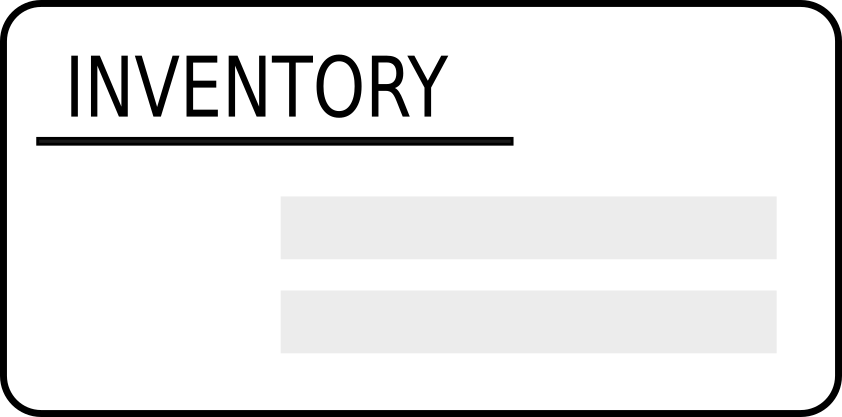
\includegraphics[width=0.80\textwidth]{images/character_inventory.png}
\end{column}
